%\documentclass[defaultstyle,11pt]{thesis}
%
%\usepackage{amssymb}		% to get all AMS symbols
%\usepackage{amsmath}		% to get equations to work right
%\usepackage{graphicx}		% to insert figures
%\usepackage{hyperref}		% PDF hyperreferences?? [backref=none]
%\usepackage{natbib}
%\usepackage[usenames,dvipsnames]{color}
%%% To make \href colors more decent:
%\definecolor{MyDarkBlue}{rgb}{0,0.1,0.7}
%\hypersetup{pdfborder={0 0 0},colorlinks,breaklinks=true,
%  urlcolor={MyDarkBlue},citecolor={MyDarkBlue},linkcolor={MyDarkBlue}
%}


\chapter{Optimized Deceleration}

Over the past two decades, Stark deceleration has enabled groundbreaking collisional~\cite{Sawyer2011,Kirste2012,Gao2018} and spectroscopic~\cite{Veldhoven2004,Hudson2006,Lev2006,Fast2018} studies of a variety of species~\cite{VanDeMeerakker2012}. 
Subsequent trap-loading greatly enhances interrogation time for such studies~\cite{Sawyer2008} and opens the door for further cooling and manipulation~\cite{Stuhl2012evap, Reens2017}. 
Zeeman deceleration has developed in parallel and enabled similar achievements for paramagnetic species. 


\section{Canonical Decelerator Geometry}

Much like related work in charged particle accelerators, a neutral particle decelerator is required to satisfy two key principles:
\begin{enumerate}
\item A particular candidate particle known as the synchronous molecule must be manipulated as desired by the device, e.g. slowed from $800-50$~m/s.
\item Other particles of similar initial conditions to the synchronous molecule must also possess similar final conditions.
\end{enumerate}
This second principle is known as phase stability, and is crucial to the overall performance of the device as far as flux or brightness is concerned.

Neutral particle decelerators face an incredible setback relative to charged particle accelerators, in that it is vastly harder to apply forces on them.
Specifically, the device I will soon describe can accelerate hydroxyl radicals at $\sim 200$~km/s/s. 
If hydroxyl cations were instead placed in the largest electric fields generated by the device of about $100$~kV/cm, they would experience an acceleration given by:
\begin{equation}
\frac{q_e\cdot E_\text{max} }{m_\text{OH}} = 5.5\times 10^9\text{ km/s/s}.
\end{equation}
This constitutes a factor of over ten million. 
But is this truly fundamental, or technically limited? 

Applying forces on neutral particles requires the application of gradients in electric field magnitude, and the magnitude of these gradients depends on the miniaturization of the geometry the electrodes.
It becomes challenging to develop a truly fair comparison, but underneath all of the details about electrodes and geometries, electric fields are always generated by charged particles, regardless of whether they are conduction band electrodes in some material.
The force on a neutral particle by a charged one scales as $r^4$, while that between charged ones scales as $r^2$.

In any case, once the factor of ten million setback is taken into account, neutrals have the nice property that only the magnitude of the field influences them, and not the direction. 
This makes it possible to generate large magnitude electric fields with the direction of the field orthogonal to the beamline, which is precisely the trick utilized in the first Stark decelerators~\cite{Bethlem1999}.
The design of this decelerator was replicated here in the Ye group, first at a length suitable for expansion with Xenon, then later with Krypton, and most recently with Neon.
Pairs of cylindrical pins are arranged alongside the beamline, so as to apply a large but localized field magnitude across it for maximum field magnitude gradient.
Successive pairs are rotated ninety degrees relative to one another, which is relevant to transverse confinement, and every fourth pin is connected up to the same backbone electrode.

\begin{figure}[ht!]
\centering
\label{decelcartoon}
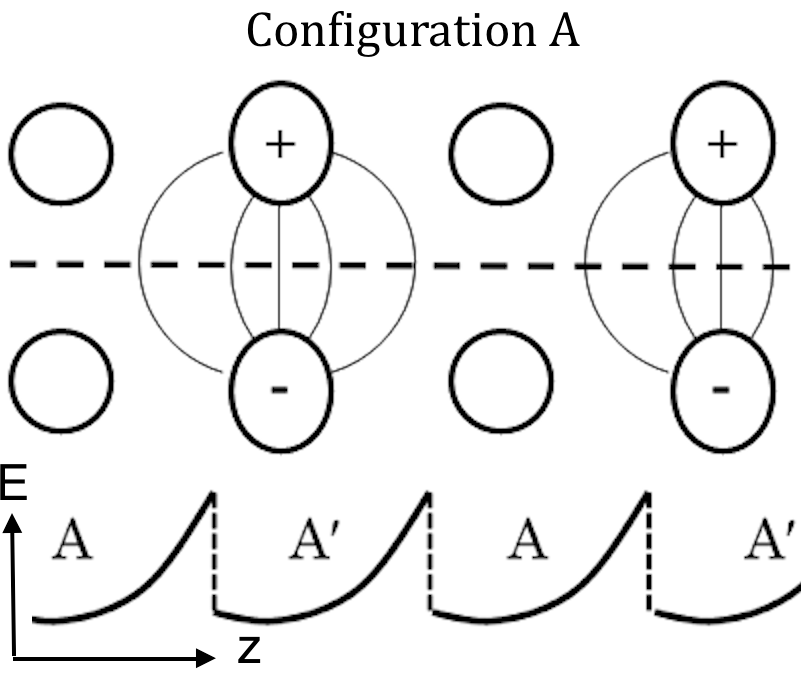
\includegraphics[width=8cm]{Slowing/chargecartoon.png}%
\caption{
Voltages, electric fields, and on-axis potential energy in a conventional pin decelerator~\cite{Bethlem1999}. Pin rotation indicated by representation as slight ellipses rather than circles. Electric fields density corresponds to the potential experienced by molecules. The horizontal dashed line indicates the central axis of the device, and the potential energy of the target or synchronous molecule as it transits this axis is shown below the pin pairs. A' indicates the translation (and rotation) of the drawn configuration of fields and voltages to the next pin pair(s). 
}
\end{figure}

Diagrams such as that shown in Fig.~\ref{decelcartoon} are useful in understanding the operation of the device.
Molecules approach a region of strong electric field, exchanging kinetic energy for internal potential energy in the case of those whose quantum state features a positive Stark shift, the only ones capable of being manipulated by such a device.
At some point, the strong electric fields are turned off, and a different region of strong electric field is turned on further along the beamline.
If the strong fields are turned off before the synchronous molecule reaches the strongest fields, i.e. partway up the hill, phase stability is obtained, because a molecule that is ahead of the synchronous one will therefore exchange a greater quantity of kinetic energy for potential energy by climbing farther up the hill before the turn-off event.
This molecule thus experiences a force restoring it to the location of the synchronous molecule.
Of course if a molecule is too far ahead, it may pass all the way through the region of highest field prior to the turn-off event. Such a molecule is no longer phase stable and will travel farther and farther from the synchronous molecule.
Thus there is a tradeoff between the deceleration capability of the device and the volume of its phase stable region.

\begin{figure}[t!]
\centering
\label{variousphaseangles}
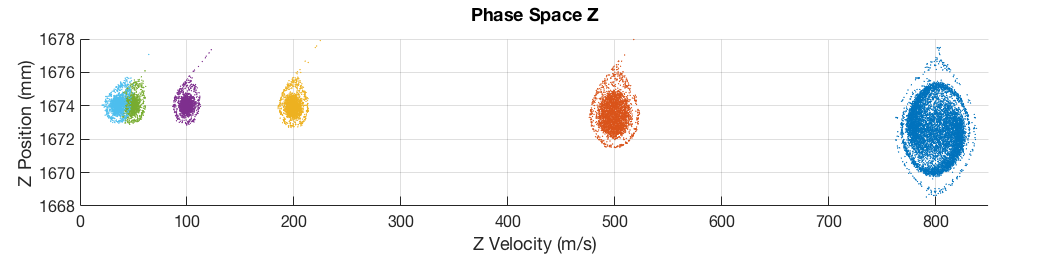
\includegraphics[width=\linewidth]{Slowing/phaseangles.png}%
\caption{
Longitudinal phase space plots of a Stark decelerator with varying final velocity. From left to right, $v_f=33, 50, 100, 200, 500, 800$~m/s. Note how the size of the populated area reduces as the final speed is reduced.  This is a direct reflection of how closely the synchronous molecule approaches the charged pin-pair, which in turn controls how far ahead a nonsynchronous molecule may be while still experiencing a restoring force. Note also how the size reduces much more significantly between $800-500-200$~m/s then for any of the other speed reductions. This is described further in the main text. 
}
\end{figure}

This can be seen more directly from simulations of its behavior, such as in Fig.~\ref{variousphaseangles}. The area of the region populated by molecules reduces as the deceleration is increased.
However, the change in area seems to plateau and then stop, somewhere between $200-500$~m/s since all velocities below $200$~m/s show nearly the same area.
This can be attributed to the fact that all of these low speeds require nearly the same energy to be removed per stage of the decelerator, since the total energy removed can be calculated by the potential energy difference:
\begin{equation}
\Delta\text{PE}=\frac{1}{2}m_\text{OH}\left(v_i^2-v_f^2\right).
\end{equation}
Once $v_f << v_i$, $\Delta\text{PE}$ no longer various strongly with $v_f$:
\begin{equation}
\label{slowphasevary}
\Delta\text{PE}\sim\frac{1}{2}m_\text{OH}v_i^2\left(1-\left(\frac{v_f}{v_i}\right)^2\right).
\end{equation}

An important corollary of this idea relates to the parameterization typically used for specifying decelerator operation.
Since the devices are periodic, it is convenient to parametrize the longitudinal coordinate with an angle, called the phase angle, and chosen to vary by $180^\circ$ between one pin-pair in the next, so that a single voltage configuration applied to the backbone repeats itself after $360^\circ$.
This parametrization also allows us to work independently from the choice of pin size and pin spacings for a given device.
A decelerator is often operated so that a synchronous molecule with a given speed would always experience a turn-off event at the same phase angle $\phi$, which then allows the operation of the device to be specified by only that angle.
It follows from Eq.~\ref{slowphasevary} however that very slight changes in $\phi$ can lead to dramatic changes in the final velocity of the synchronous molecule.
In earlier iterations of the code used for programming the switching sequence of our decelerators, it was necessary to specify the phase angle down to the thousandth of a degree in order to get the desired final speed within a few meters per second, which in turn required carefully hand-exploring the function mapping phase angles to final speeds.
This is discussed further in an appendix.

It is also worth discussing some other features of the longitudinal phase space plots shown in Fig.~\ref{slowphasevary}. 
Almost all final speeds show a bullseye type pattern, with a halo of outer particles surrounding an inner core.
This is discussed extensively in~\cite{VanDeMeerakker2006}, and relates to a discussion of inefficiencies in the device that will be continued in the next section.
However, there is additional structure evident within the inner core, especially for the molecular packet with $800$~m/s final velocity.
These molecules have not had their speed modified significantly by the simulated device, in which case the activity of the device is better described as ``bunching'' the molecules than ``slowing'' them.
In the experiment, these bunched molecules would travel together with a large population of unaddressed molecules with initial longitudinal velocity and position unsynchronized with the timing of the device.
These unaddressed molecules are nonetheless transversely focused, and in some cases with better efficiency than target molecules, and so constitute a rather large background signal relative to the molecules of interest.
The reason these unaddressed molecules are not evident in this simulation is that the simulation only initializes molecules that are likely to be addressed, for reasons of runtime.

This in turn relates to the substructure evident in the inner core of the bunched molecules in Fig.~\ref{slowphasevary}.
This substructure is an artifact of incomplete phase space filling in the simulation, i.e. if the right molecules had been included in the initialization, the inner core would be uniformly filled out and not feature any swirling.
It is useful to keep an eye out for such artifacts as a way of monitoring whether the initialization assumptions of a simulation is valid. 
This swirling is not necessarily only an artifact however, and can in fact be relevant in the experiment as well.
In~\cite{Parazzoli2009}, the rotating nature of the inner core in phase space is intentionally understood and exploited for minimizing the velocity spread of a beam exiting a decelerator.

\section{Alternative Geometries and Configurations}

Alongside the history of achievements enabled by Stark deceleration runs a parallel ongoing saga surrounding their efficient operation. 
Many important steps have been made, not only in understanding the flaws of the canonical pulsed decelerator~\cite{VanDeMeerakker2006,Sawyer2008a}, but also in addressing them through the use of overtones~\cite{VanDeMeerakker2005a,Scharfenberg2009}, undertones~\cite{Zhang2016}, or even mixed phase angles~\cite{Parazzoli2009,Hou2013}. 
Even with these advances, the outstanding inefficiencies of the pulsed decelerator, particularly with regard to transverse phase stability, have motivated alternative geometries such as interspersed quadrupole focusing~\cite{Sawyer2008a} and traveling wave deceleration~\cite{Osterwalder2010,VandenBerg2014,Fabrikant2014}. 
Although traveling wave deceleration takes a strong step in the right direction toward truly efficient operation, it comes with costs in system complexity and high voltage engineering. 
These costs can be partially addressed by the use of combination pulsed and traveling wave devices~\cite{Quintero-Perez2013}, or even using traveling wave geometry with pulsed electronics~\cite{Hou2016,Shyur2017}. 
Others continue to pursue brand new geometries aiming to enhance transverse acceptance without abandoning more reliable pulsed electronics~\cite{Wang2016}. 

\subsection{Flaws in Canonical Deceleration}

I begin here by describing more precisely these flaws in the canonical pulsed decelerator.
It is useful to distinguish between two primary categories of performance breakdown:
\begin{enumerate}
\item Breakdown associated with the discontinuous nature of the geometry.
\item Breakdown associated with the nature of the phase stable region.
\end{enumerate}
The first breakdown mechanism follows directly from the geometry of the canonical pulsed decelerator. Focusing only occurs in a given transverse direction every other pin pair. So if the speed of the beam is decreased enough, there is clearly a point at which molecules will be adversely effected.
The same issue exists for the longitudinal direction. Switching events are required for molecules to experience restotring force in the longitudinal direction. When molecules do not encounter pin pairs with enough frequency, molecules again are adversely affected.
Discontinuity breakdowns are thus further classified by their transverse and longitudinal manifestations- overfocusing and reflection loss- discussed further in~\cite{Sawyer2008a}.
These breakdowns can in general be described by a lower bound on the velocity of the beam:
\begin{equation}
v_z >> Lf_\text{osc} \label{breakdownequation},
\end{equation}
where $z$ indicates the propagation direction, $L$ indicates the distance between successive pairs of pins, and $f_\text{osc}$ is the oscillation frequency of the molecules about the synchronous molecule.
This latter parameter is not strictly well defined across the entire ensemble, but accepts a range of possible values according to the anharmonicity of the restoring force experienced by molecules with different deviations from the synchronous molecule.
For typical operating conditions, $f\sim 1-2\text{ kHz}$.

\begin{figure}[t!]
\centering
\label{bunchingphasespace311}
\includegraphics[width=\linewidth]{Slowing/many-bunching-plots.png}%
\caption{
Longitudinal phase space plots after several types of bunching for several decelerator lengths. Column-wise, operation is in $S=1$, $S=3$, and $S=311$. Indicated percentages are comparable by rows, but suffer from a pernicious simulation artifact. Some molecules are included which actually pass through decelerator pins. The effect adversely influences the comparative survival numbers, but not the observed projection of phase space onto the longitudinal direction.
}
\end{figure}

This anharmonicity is at the core of the second kind of breakdown in performance of the pulsed decelerator, a breakdown which results in unwanted decreases in the flux of the device even without any of the issues associated with low final speeds.
In fact, the effect is already clearly manifested for devices operated in bunching mode without any slowing, refer to Fig.~\ref{bunchingphasespace311} for the following discussion.
One way to understand these flaws is to think in terms of an unwanted coupling between transverse and longitudinal modes~\cite{VanDeMeerakker2006}.
In words, molecules are best focused transversely on their closest approach to the charged pin pair, and therefore molecules which deviate significantly from the synchronous molecule in the longitudinal direction experience the best transverse focusing.
It follows that the two directions of motion are strongly coupled to one another, and any full description of their equations of motion will not be separable.
It also follows that molecules would survive better at greater distance from the synchronous molecule in longitudinal phase space, which agrees nicely with the observed sparsity close to the center of the left four plots in Fig.~\ref{bunchingphasespace311}.
The dead band and outer ring are best explained in terms of parametric amplification phenomena~\cite{VanDeMeerakker2006}.

One way to address this is to allow the molecules to pass all the way through a charged pin pair, and only switch the fields after they climb a second hill.
This is known as overtone operation~\cite{VanDeMeerakker2005a}, where the term stems from the fact that even without intending it, the standard operating mode supports overtone operation for molecules that happen to begin at triple the intended speed.
Or one may intentionally reduce the switching frequency by a factor of three, typically indicated by the overtone parameter $S$ as $S=3$ operation, in which case standard operation may be referred to as $S=1$.
This gives rise to the much more homogeneous set of phase space plots in the center column of Fig.~\ref{bunchingphasespace311}.
Despite improved homogeneity, the plots are thinner than those for $S=1$ by a factor of $\sqrt{3}$, which stems from the fact that molecules experience restoring force in the longitudinal direction with one third frequency. 
They can therefore deviate from the synchronous molecule by only a third as much kinetic energy as before, or $1/\sqrt{3}$ less deviation in velocity.
An even more important drawback of $S=3$ operation is that only a third as much energy may be removed per unit distance.

It is also possible to use a hybrid approach that we term $S=311$.
In this operating mode, one allows the synchronous molecule to climb all the way over a hill only every third time.
It should be noted that $S=31$ operation, where the synchronous molecule climbs all the way over a hill every other time, is not as useful because this molecule would only experience extra focusing in one of the transverse directions.
This mode has the advantage of sacrificing less deceleration capability, since it is $60\%$ as effective as $S=1$ since $3/5$ of all possible hills are climbed, but also addressing some of the coupling issues.
As can be seen in the last column of Fig.~\ref{bunchingphasespace311}, the sparsity closest to the synchronous molecule at the center of the phase space is addressed, although a parametric amplification dead band still persists.
Unfortunately this mode also features an increased sensitivity to low speeds.
Typically, $S=1$ operation stops performing due to low speed breakdown below $50$~m/s, and $S=3$ below $150$~m/s.
The cutoff has not been studied thoroughly for $S=311$, but a hybrid alternative exists, which is to use $S=311$ for the bulk of the deceleration except when the speed drops below $150$~m/s, at which point one returns to $S=1$ for a brief enough time that the transverse-longitudinal coupling does not lead to excessive loss.
In practice, this has yielded factor of $2-3$ improvements in the number of molecules which may be slowed or trapped in our experiment.

\subsection{Alternative Geometries}

Perhaps the most important class of alternative geometries for deceleration are those that are continuous in nature. 
These include both Stark~\cite{Osterwalder2010} and Zeeman~\cite{Narevicius2008} varieties, and in principle provide a complete solution to breakdowns associated with the discontinuous nature of pulsed geometries, although in practice they face various low-speed challenges of their own.

The Stark devices, also known as traveling wave decelerators, feature cylindrical symmetry and use sinusoidal voltages to generate a macroscopic moving trap which can be translated or decelerated, and even brought to rest, at least provided high voltage amplifiers with bandwidth down to DC operation.
The most common and as far as I can tell the only geometry used thus far, in three or four different groups, is that described in~\cite{Osterwalder2010} with $0.8$~mm diameter wires bent into $4$~mm inner diameter rings, and connected up to eight different backbone electrodes.
Their total phase space acceptance, at least for lower decelerations, is an incredible improvement over $S=1$ operation, skip ahead to Fig.~\ref{modescomparedefftrap} and compare $S=1$ to $TW$ in panel (b).

There also exist a host of proposals for alternative pulsed geometries, including this one with interspersed quadrupole focusing stages~\cite{Sawyer2008a}, this one with charged wires for improved transverse behavior~\cite{Wang2016}, and even a magnetic device with interspersed hexapole stages for use with NH molecules~\cite{Plomp2019}. The first two may become less important thanks to the results discussed in the next section.

\subsection{Alternative Field Distributions}

We mix alternate field distributions into the deceleration scheme that feature strong restoring force in the transverse directions, refer to Fig.~\ref{fig:chargecartoon}.
%This restoring force averages into the effective moving trap, leading to the dramatic improvements over S=1 shown in Fig.~\ref{fig:efftrap}. 
In the canonical S=1 operating mode~\cite{VanDeMeerakker2012}, molecules approach a charged pin-pair, climbing a hill in potential energy. 
The hill is abruptly switched off partway up the hill, allowing molecules to have phase stability as discussed above.
But it follows that molecules spend a significant portion of their flight passing between grounded pins.
Conventionally, pins are always charged in bipolar pairs, in which case few field lines run toward the grounded pin-pairs, and those that do create a slight defocusing effect. 

\begin{figure}[t!]
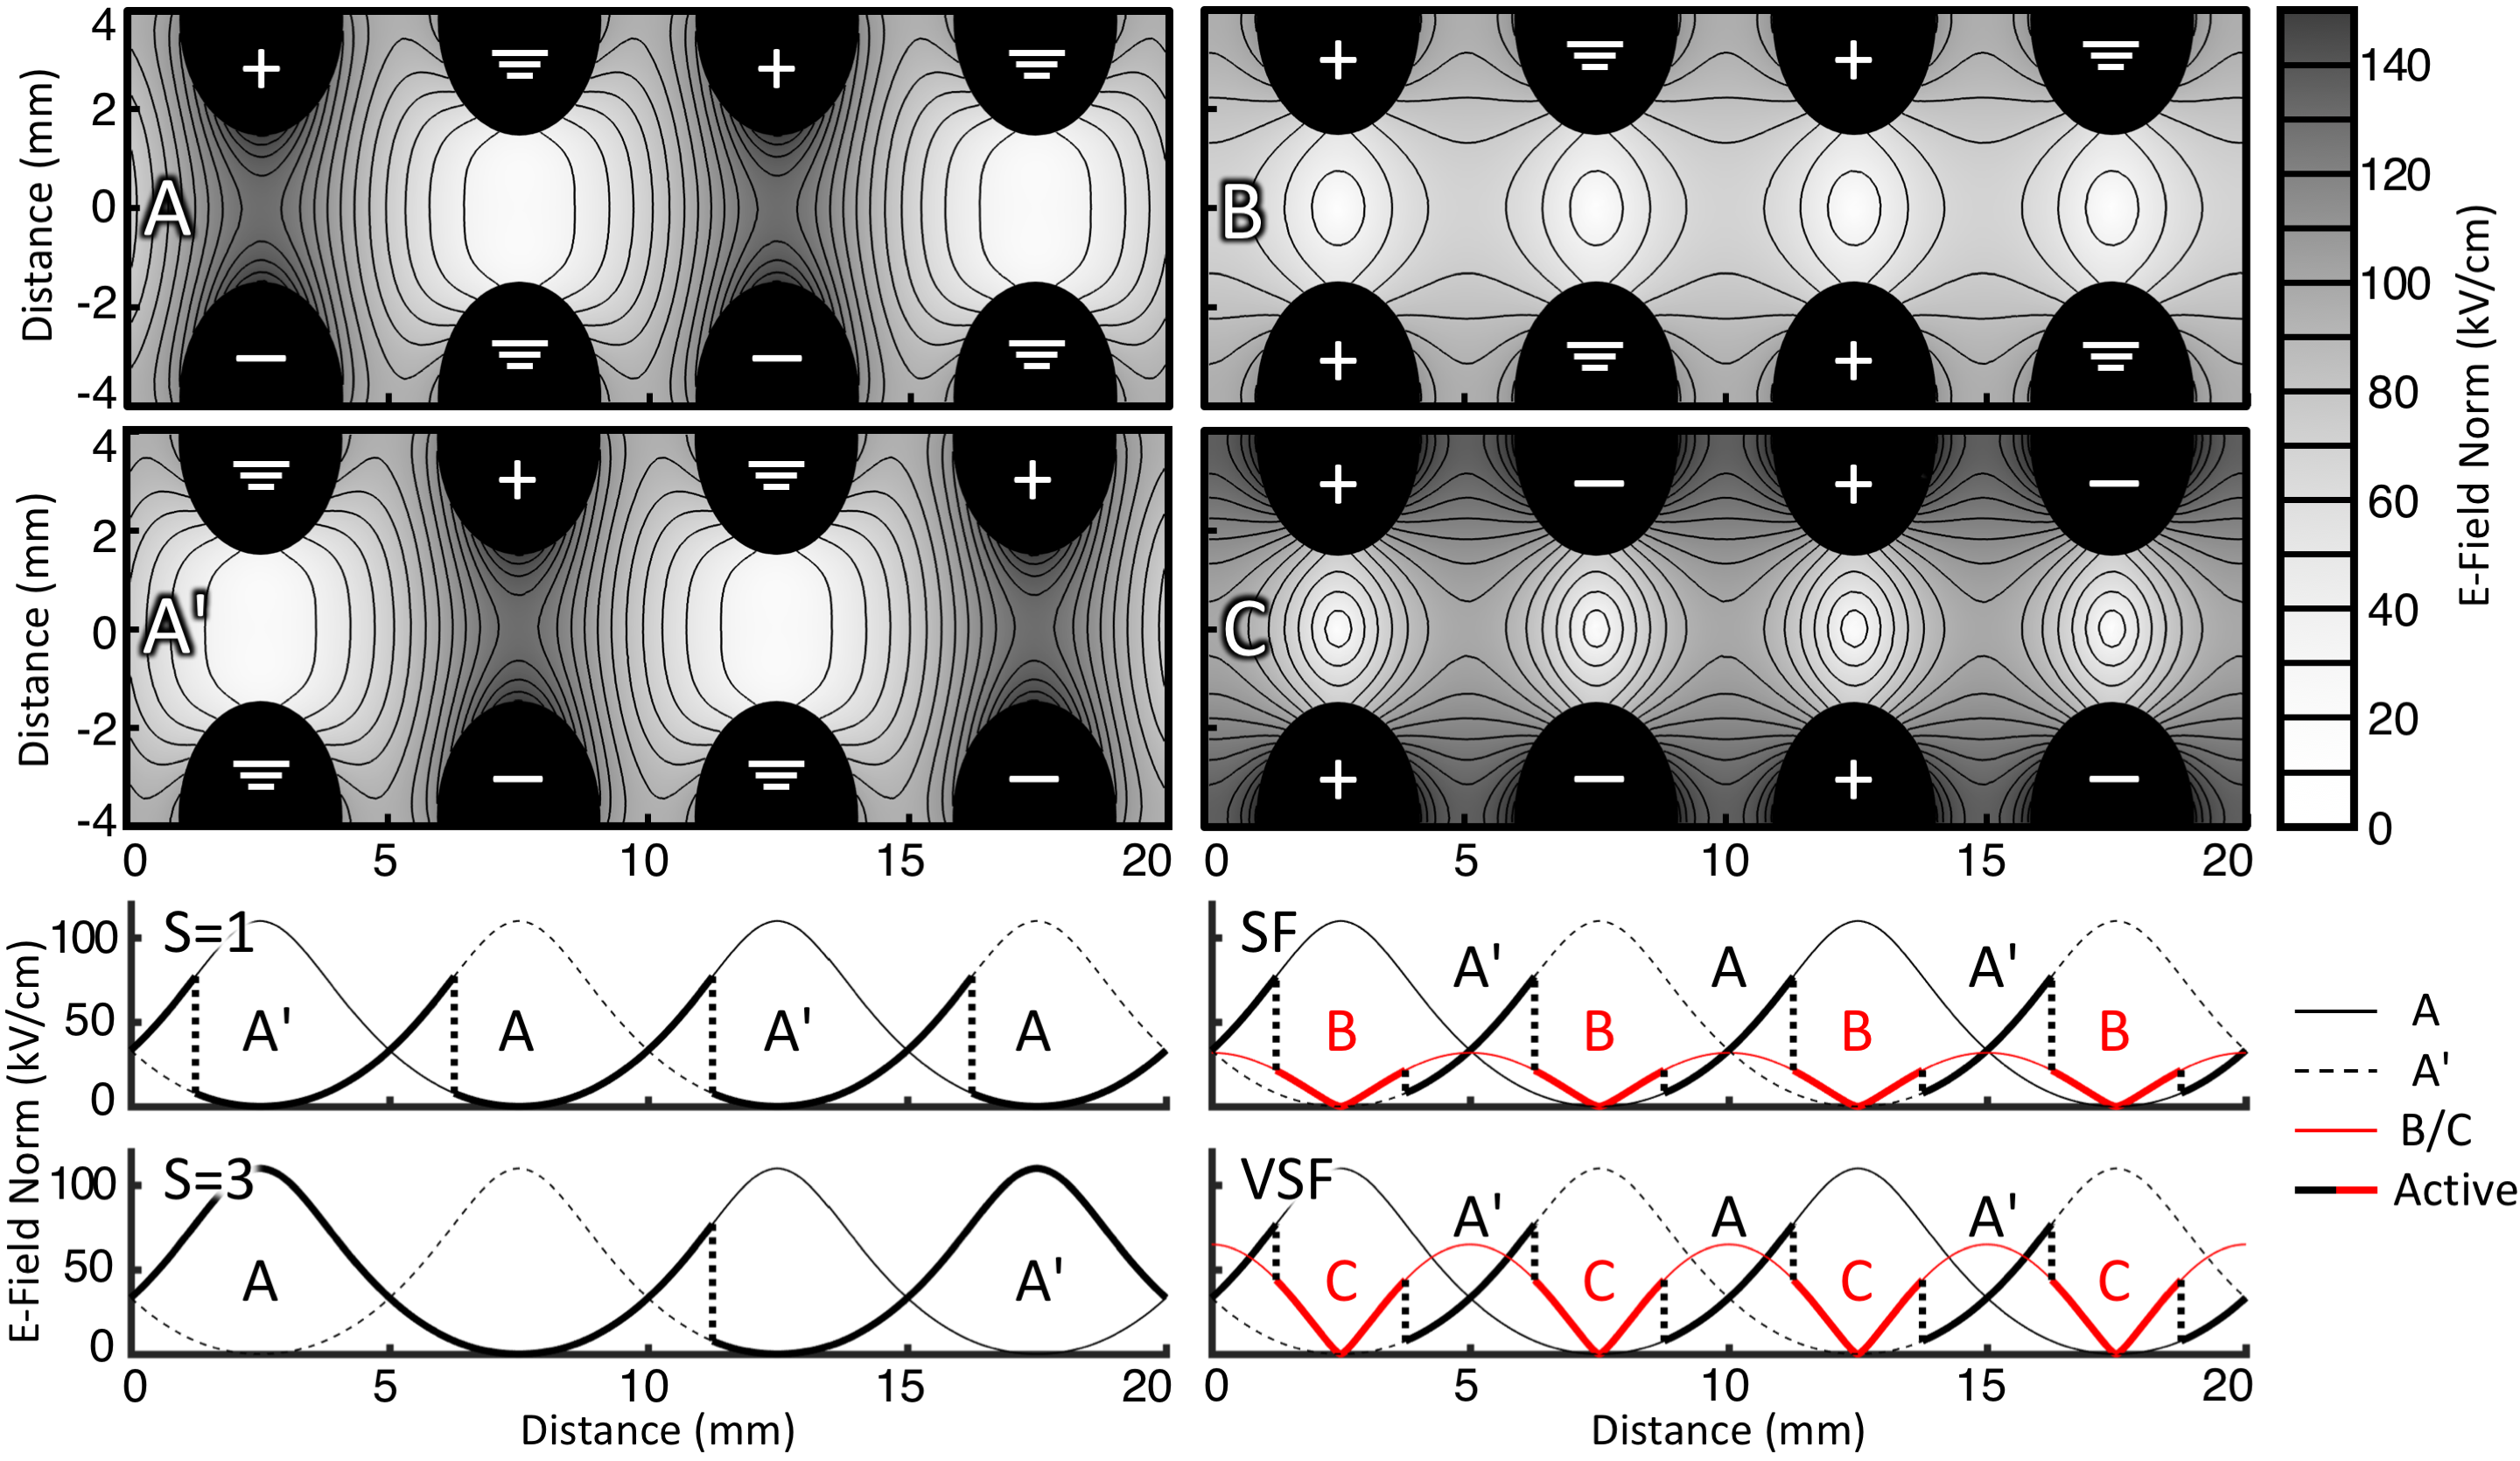
\includegraphics[width=\linewidth]{Slowing/pinpairformal.png}%
\caption{
This schematic illustrates alternate voltage configurations which can be used alongside the conventional one for greatly enhanced performance. Configurations B-D feature strong transverse focusing in the regions where molecules would normally pass between grounded pin pairs. On-axis energy diagrams are shown for several modes of operation incorporating these alternate configurations, with primes indicating translation to the next pin pair. In addition to S=1 mode and its S=3 overtone~\cite{VanDeMeerakker2005a}, a strong focusing (SF) and a very strong focusing (VSF) mode are introduced. Equipotentials of the effective trap during $\phi=45^\circ$ slowing are shown, with units appropriate for hydroxyl radicals.\vspace{-4mm}
}
\label{fig:chargecartoon}
\end{figure}


Useful alternate configurations can be created by applying voltage in a way that is not balanced between adjacent pin pairs. 
Once an imbalance exists, by charging up both pins in a pair to the same non-zero voltage, by only charging one pin in a pair, or even by unbalancing the decelerator power supplies~\footnote{It was once noted that imbalancing the power supplies led to improved performance on a conventional pulsed Stark decelerator. S. Hoekstra, private communication.}, the field lines will run between pin-pairs. 
Near the grounded pin-pair, these field lines create a focusing 2D quadrupole structure, much like this one used intentionally for trapping and controlling spin-flip losses~\cite{Reens2017}. 
By implementing these configurations when the synchronous molecule is flying between the grounded pin pair, but retaining the use of the conventional configuration for hill climbing, the longitudinal behavior of the device is unaffected while the transverse behavior is vastly improved.
Regarding spin-flip losses, use of these configurations is cause for concern, but not significant as far as early modeling is concerned. This is discussed further towards the end of this chapter.
Utilizing the alternate configuration of charging both pins in a pair to the same voltage gives rise to a new strongly focusing operation mode (SF), and utilizing the configuration where the adjacent pin pair gives a very strongly focusing mode (VSF). 
It is also possible to obtain some of these effects without the need for rods being charged to three different voltages, by making use of the field distribution generated by turning on only a single pin, a somewhat focused mode (F).
This is especially significant for being realizable immediately on existing devices with no new electronics, and offers 4-fold gains at trappable speeds, see Fig.~\ref{speedvary}. 

\subsection{The Effective Moving Trap}
In order to quantitatively analyze these and other operation modes, we can work in the non-inertial moving frame of the molecules, where any feasible mode generates an effective trapping potential with deceleration included as a fictitious force. 
%One of the key motivations for improvement of the conventional pulsed decelerator operation are its well-known failings as far as phase-space stability is concerned. These have been described in terms of transverse-longitudinal couplings~\cite{VanDeMeerakker2006}, small separatrix area at high phase angles~\cite{Hudson2004}, or reflection at low velocities~\cite{Sawyer2008a}. 
This approach is usually reserved for continuous deceleration schemes~\cite{Osterwalder2010,Narevicius2008}, but is equally valid for pulsed schemes provided their velocity satisfies Eq.~\ref{breakdownequation}. 
The effective trap for on-axis molecules in the longitudinal direction has been discussed at length~\cite{Bethlem2000,Hudson2004}, but computation of the full 3D effective trap has not been reported previously.
The 3D effective trap is evaluated numerically for various operation modes to obtain the equipotential surfaces in Fig.~\ref{shapearray}.
It is found that for S=1, the effective trap has holes. 
Molecules moving away from the trap center along the $x$ and $y$ axes experience almost no restoring force at all. 
This can be considered the underlying reason for the transverse-longitudinal coupling problem discussed above. 
Such couplings are in some contexts useful for maintaining ergodicity in a trapping geometry~\cite{Surkov1996}, but with one dimension featuring a very low energy barrier, they lead to loss.

\begin{figure}[t!]
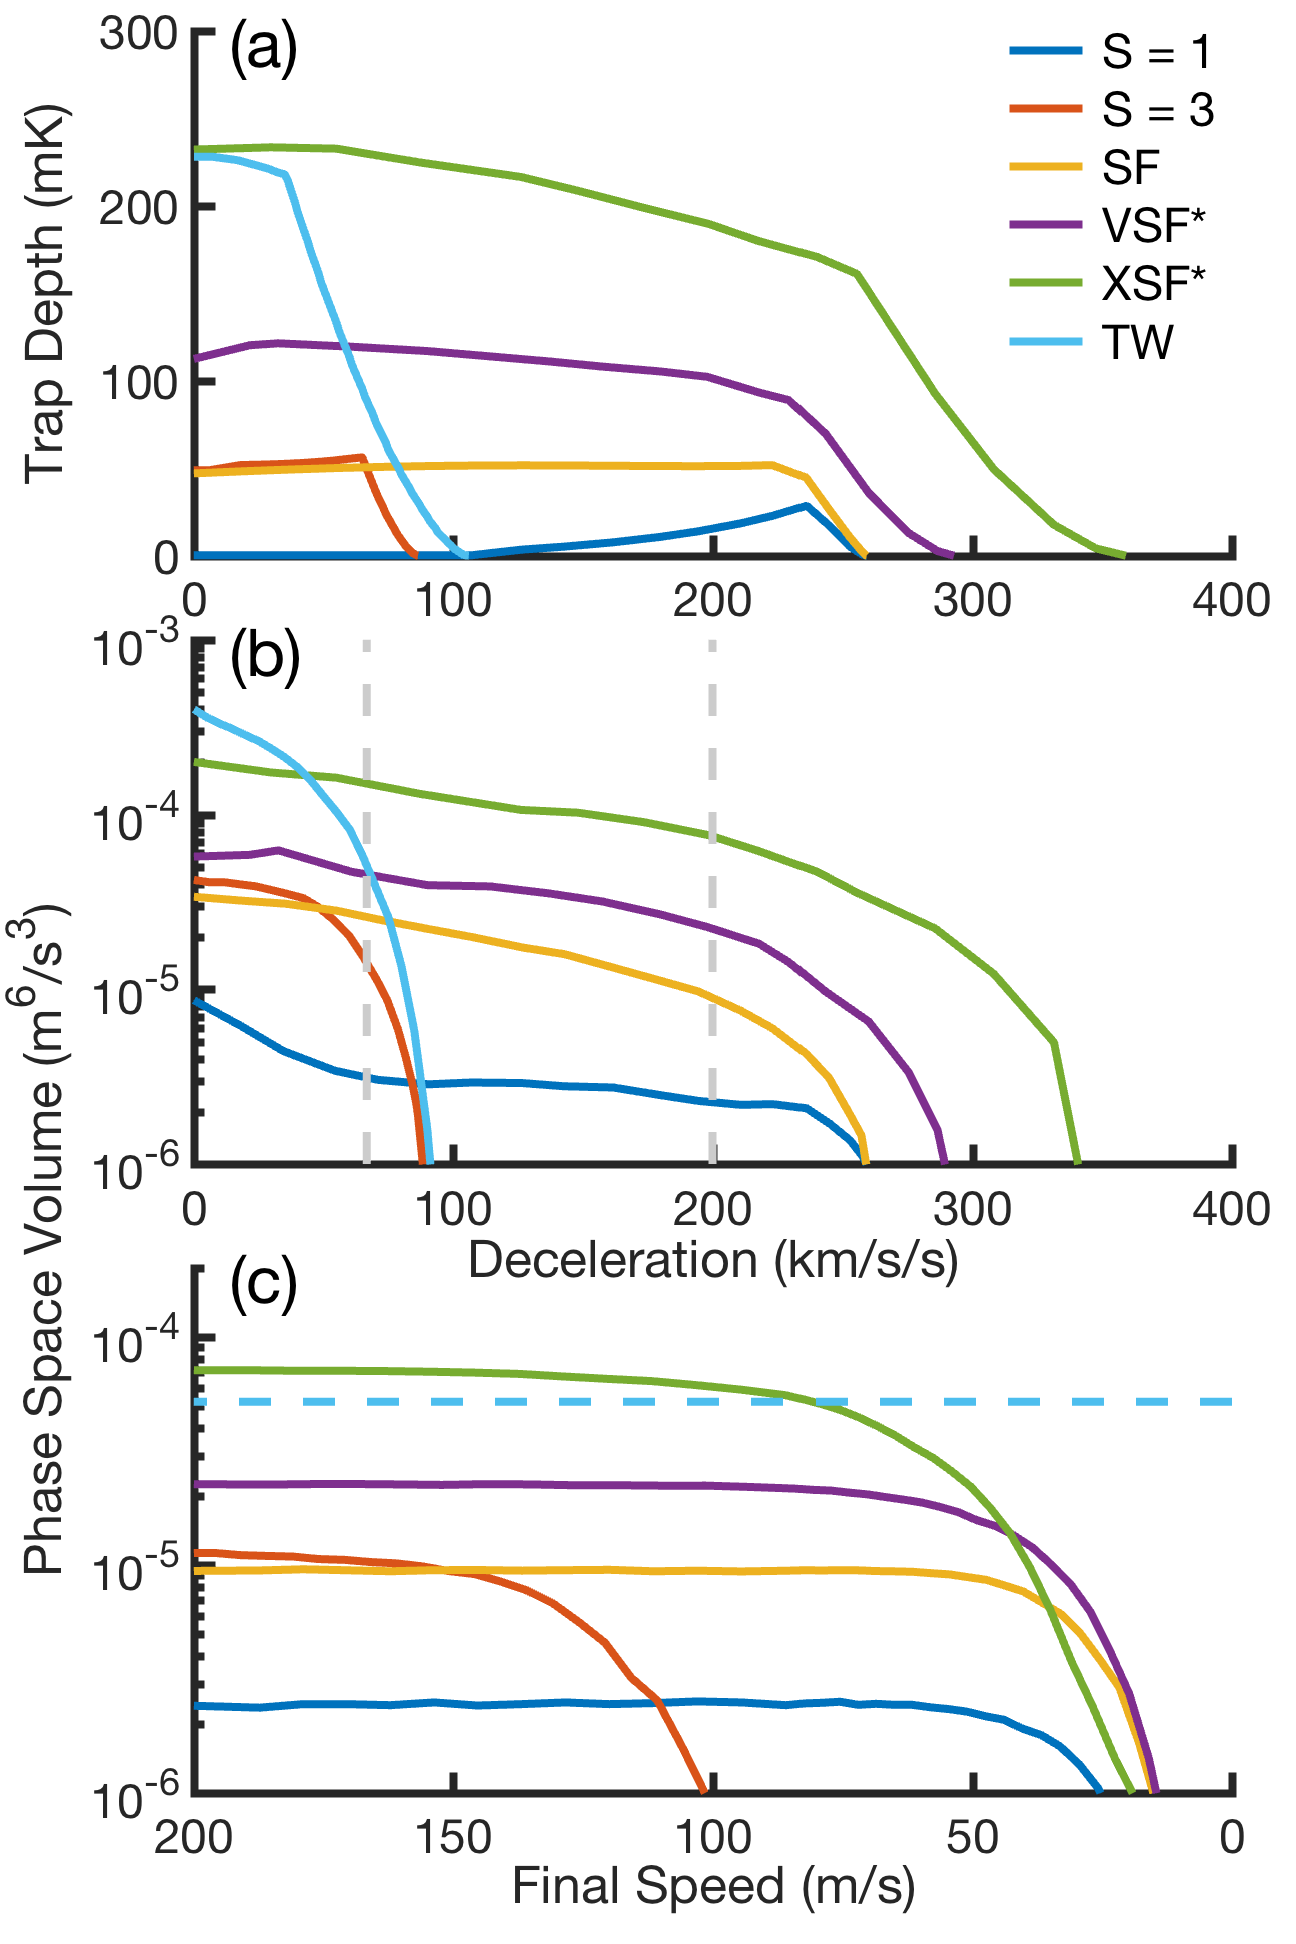
\includegraphics[width=10cm]{Slowing/full-three-panel.png}%
\vspace{-5pt}
\caption{
Characterizing the moving trap under different modes of operation. In addition to the canonical S=1 and S=3 modes, newly defined strong focusing (SF), very strong focusing (VSF), and focusing (F) modes are shown. Traveling wave (TW) deceleration is also compared, assuming $10$ kV peak to peak, to our knowledge the largest voltage used to successfully decelerate to rest with a TW device. In panel (a) the trap depth at the lowest point of escape is shown as a function of deceleration for different operating modes. In panel~(b) the initial phase space volume remaining within these effective traps after a $3$~ms hold time is shown, and in panel (c) a full decelerator simulation is performed as a function of final velocities, with hold time fixed also at $3$~ms and deceleration fixed as indicated by the gray dashed lines in panel~(b). For TW a full simulation is not performed, since low speed losses are less significant, but the dashed line shows the value corresponding to 67 km/s/s in panel (b).\vspace{-4mm}}
\label{fig:efftrap}
\end{figure}

Motivated by the holes evident in S=1 mode, a new figure of merit that may be used to compare the performance of various modes of operation is introduced: the minimum depth of their effective moving traps.
Here minimum depth refers to the smallest energy above which a molecule with that energy can find a way out of the trap.
Having a single value to characterize effective traps allows doing so systematically across many modes and across many magnitudes of the applied deceleration, see Fig.~\ref{fig:efftrap}a. Remarkably, F mode offers comparable trap depth improvement to S=3, but with no sacrifice in deceleration capability. 
The SF and VSF modes make still more dramatic improvements, with the latter even rivaling traveling wave (TW) deceleration~\cite{Osterwalder2010}. 
Note that for SF and VSF, the alternate configurations are not utilized in a symmetric manner about the grounded pin pair as for F. 
Instead, allowing them to be used asymmetrically opens up a new degree of freedom, which is optimized so as to maximize the minimum depth.

We can make further use of the effective trap by directly employing it to simulate the fate of particles confined for $3\text{ ms}$, the duration of a typical deceleration sequence (Fig.~\ref{fig:efftrap}b). 
The results show a very close qualitative match to the trends predicted by the minimum trap depth. 
The most notable exception is found in S=1 mode at low decelerations, where extremely deep holes dominate the minimum trap depth, but the small effective cross sectional area of the holes still allows molecules to survive in greater number than at higher decelerations where the minimum trap depth actually improves.
As far as the comparison with TW is concerned, it is important to point out that we use the rather small $2\text{ mm}$ pin-pair spacing and $2$x$2\text{ mm}^2$ opening area of our device, while TW devices use $4\text{ mm}$ diameter rings.
If VSF mode were used with a $3$x$3\text{ mm}^2$ device~\cite{Scharfenberg2009} or a $4$x$4\text{ mm}^2$~\cite{VandeMeerakker2005}, phase space volume would increase significantly, depending approximately on the cube of pin-pair spacing, and thus outperforming TW. 
Deceleration does also reduce linearly with pin-pair spacing, since this influences the number of pins that may be fit next to one another in a given longitudinal distance.

Of course the validity of using the effective trap in this manner depends on the final speed after the deceleration sequence.
This effect can be isolated by also performing a full Monte-Carlo simulation of the various deceleration modes, without use of the effective trap approximation.
By varying only the final speed, and keeping deceleration and run-time exactly fixed by appropriately varying initial speed and decelerator length, we obtain the results shown in Fig.~\ref{fig:efftrap}c, an exact isolation of the low speed effects from other phase space effects.
The asymptotically flat profiles at high enough speeds validate the effective trap picture, as do the quantitative agreement between the asymptotic values and the corresponding points at $200\text{ km/s/s}$ and $67\text{ km/s/s}$ in Fig.~\ref{fig:efftrap}b. 

The beginning of the low-speed breakdown depends on the intended use of the decelerator, and especially how far the molecules will be expected to travel unguided afterwards. 
In Fig.~\ref{fig:efftrap}c, the molecules still confined within a $3\text{ mm}$ diameter circle after $5\text{ mm}$ free flight after the end of the sequence are shown. 
This is a conservative representation of what is required for trap-loading, but for collisional experiments a larger flight distance may be required.
Note how F and SF cut off at even lower speeds than S=1, but VSF cuts higher. 
This can be attributed to the fact that VSF actually features an increased transverse trap frequency relative to the others, while F and SF improve over S=1 mostly by plugging holes and not by increasing the trap's depth or frequency.
This restricts the usefulness of VSF mode for OH or other strongly dipolar species at low speeds to devices that combine with a TW device as in~\cite{Quintero-Perez2013}.
For less strongly dipolar species however, VSF will more easily respect the low velocity transverse oscillation bound, and may not feature an altered low speed cutoff relative to SF or F.


\section{Trap Oscillations}

\section{HV Isolation Strategies}

\section{Manufacturing Considerations}



%\bibliographystyle{unsrtDR}	% or "siam", or "alpha", etc.
%\bibliography{allrefs}		% Bib database in "allrefs.bib"
%\end{document}